\subsection{Compression}\label{subsec:compression}
For compression, the most straightforward metric is to measure the reduction of memory required to
store the data.
To normalize over image resolution, we choose to evaluate the \ac{bpp}.

The second, and less objective measure, is image similarity after reconstruction.
While the \ac{mse} and by transfer \ac{psnr} describe pixel-wise similarity very well, it is not
always optimal to judge perceived similarity for humans, as can be seen in Figure~\ref{fig:mse_ssim}.

\begin{figure}[ht]
    \centering
    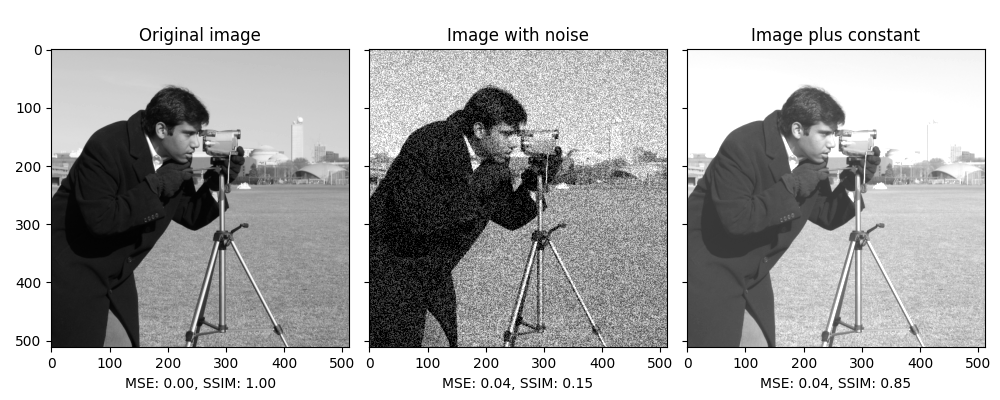
\includegraphics[width=0.8\textwidth]{images/ssim_mse}
    \caption{from~\cite{scikit-ssim}}
    \label{fig:mse_ssim}
\end{figure}

To overcome these limitations we will use the \ac{ssim}, a metric working under the assumption that human visual
perception is highly adapted for extracting structural information from a scene, that has been

Even though this analysis favours \ac{ssim}, we use \ac{mse} as our loss function for our baseline models,
since the \ac{vq} implementation we plan to replicate does the same, and we want to maximize comparability.
We use \ac{ssim} for result evaluation, and add \ac{psnr} values for further work later on.

\subsection{Image Generation}\label{subsec:image-generation}
An important metric in Image Generation and the one used to argue about the strong performance of the \ac{vq} in the
paper is the \ac{nll} normalized to the amount of pixels (dimensions) in an image, given in bits/dim.
A lower number indicates a higher likelihood of generating the test data given our model.
The bits/dim number is rooted in information theory, and describes the average number of bits required to
compress the test data with the entropy coding scheme that is optimal for a model~\cite{shannon}.

The \ac{fid}, introduced by~\cite{fid}, is another interesting metric.
It compares the distribution of features of a generator with that of real images via a network trained on a big
dataset, often also imagenet.

Another criterion not to be left out is the classic human turing test, as in evaluating the images by hand.
Even though this is not scalable, it is the ultimate classifier for human perception, and can be a good starting
point.

As on metrics we found, but decided not to use: The paper that introduced \ac{fid} it also shows that it is more
consistent than a previous, similar metric, the inception score, which we will therefore leave out.
Another sometimes utilized evaluation metric that research has shown to better avoid are Parzen Windows Estimates~
\cite{note_on_eval}.

Overall, since we have not yet implemented any Image Generation functionality, it remains to be seen which of these
criteria are of which worth to us.

TODO: INTRODUCE FORMULAS FOR THE CRITERIONS

\subsection{Class differences}

\subsection{Good Features}\label{subsec:good-features}
In classical machine learning, a set of features is ``good'', if it helps the
model to achieve a certain task.
This implies that the features should be
informative, meaning that they should have some predictive value towards our
final goal.
In simple regression settings, this is the case if the feature
correlates with the true value.
Furthermore it is helpful for features to be
independent form each other.
Dependent features could overemphasize their
importance due to the higher frequency.
And lastly, features should be simple.
A classical example would be the task of delivery time prediction between two
locations.
Here it is advised to use the distance between the two locations
instead of passing a pair of coordinates, which would cause the model to first
extract knowledge about the distance of the locations.
Another important thing
to think of is normalization.
Features that intrinsically live on a scale
magnitudes larger than other features will have higher impact on the final
output and will therefore be considered ``more important'' than other features.

The above listed reasons all are due to the fact that traditional ML models
usually are very sensitive to small perturbations which calls for efficient
feature engineering.
In modern deep learning settings this is not so much the
case.
Here we see that the models generally become insensitive to small
perturbations in the data.
Thats why there is generally not much preprocessing done.
Most commonly the data is normalized into a [-1, 1] range.
